\chapter{Supersymmetry and Grand Unification: Lecture 2}

This lecture approaches supersymmetry by backing away from it. Before we can speak sensibly about a symmetry relating bosons and fermions, we first have to understand a peculiarity of fermions themselves: they remember a full \(2\pi\) rotation. From there the lecture moves to exchange symmetry, then to the sign of closed loops, and only then to the zeroth-order supersymmetric idea that bosons and fermions may come in partner pairs whose dangerous quantum corrections cancel.

The progression matters. The lecture does not present supersymmetry as a formal algebra dropped from the sky. It constructs the need for it step by step: a topological oddity of rotations, an experimentally meaningful minus sign, a minus sign for closed fermion loops, and finally the hope that opposite-sign bosonic and fermionic corrections might tame vacuum energy and boson self-energies. The lecture closes by turning the whole story around and asking what an exactly supersymmetric world would actually look like. The answer is: not like ours.

\section{Rotations, \(2\pi\), and Topological Memory}

The lecture begins with a deliberately unsettling claim: a rotation by \(2\pi\) is not, in the relevant topological sense, the same thing as doing nothing. The geometric image is a ball in a box, with strings connecting the ball to the walls. The box is to be thought of as spatial infinity, so it must remain fixed. If the ball is rotated by \(2\pi\), the strings are tangled; by \(4\pi\), the tangle can be undone. We do not prove that theorem here in any formal homotopy language. The point of the construction is to establish that \(2\pi\) is not quite innocent, while \(4\pi\) is.

That geometric memory is then transferred to quantum states. We imagine that position is held fixed and that only spin remains. Let \(\ket{\psi}\) denote the spin state. The simplest possibility is that a \(2\pi\) rotation acts only by multiplication with a number:
\begin{equation}
R(2\pi)\ket{\psi}=\xi\ket{\psi}.
\end{equation}
The lecture then leans on the topological statement that a \(4\pi\) rotation is equivalent to doing nothing. Applying the same operation twice,
\begin{equation}
R(4\pi)\ket{\psi}=\xi^2\ket{\psi}=\ket{\psi},
\end{equation}
so we must have
\begin{equation}
\xi^2=1,
\qquad
\xi=\pm 1.
\end{equation}

At this point the distinction between bosons and fermions enters in its most elementary form:
\begin{equation}
R(2\pi)\ket{\psi_{\mathrm{boson}}}=+\ket{\psi_{\mathrm{boson}}},
\qquad
R(2\pi)\ket{\psi_{\mathrm{fermion}}}=-\ket{\psi_{\mathrm{fermion}}}.
\end{equation}
Operationally, the lecture imagines implementing such a rotation with a magnetic field. One can rotate the field itself, or let the spin precess in the field. The laboratory detail is not the point; the point is that a \(2\pi\) rotation is a meaningful operation on spin states, and that bosons and fermions respond differently.

\section{Spin States and the Interference Test}

A global minus sign ordinarily looks unphysical. If the entire wavefunction is multiplied by \(-1\), every probability computed from \(\Psi^*\Psi\) is unchanged. The lecture therefore pauses over the obvious question: if a fermion picks up a minus sign under a \(2\pi\) rotation, can that sign ever be detected?

\subsection{Question \& Answer}

Yes, but only relatively.

The lecture answers by using a two-path interference experiment. We split a single-electron wavefunction into two branches,
\begin{equation}
\Psi=\psi_1+\psi_2.
\end{equation}
Now imagine that only one branch enters a region in which the spin is rotated by \(2\pi\). For a fermion, that branch changes sign. If \(\psi_1\) is the rotated branch, then after the rotation
\begin{equation}
\Psi'=-\psi_1+\psi_2.
\end{equation}
Up to an overall irrelevant sign, the physical distinction is between the even and odd combinations,
\begin{equation}
\psi_1+\psi_2
\qquad \text{versus} \qquad
\psi_1-\psi_2.
\end{equation}

This is now experimentally visible. If the two returning wave packets are mirror images of one another about the center of the screen, then the odd combination must vanish there:
\begin{equation}
\Psi_{\mathrm{odd}}(0)=0.
\end{equation}
So a relative minus sign shifts the interference pattern; maxima become minima. By contrast, if both branches are rotated together, the total state changes only by an overall sign, and then nothing observable changes:
\begin{equation}
|\Psi|^2 = (-\Psi)^*(-\Psi).
\end{equation}

The lecture lingers here for a good reason. It is not enough to say that fermions pick up a minus sign under \(2\pi\). One must also see how that sign becomes real physics. The answer is that absolute phases remain hidden, but relative phases do not.

\section{Exchange Symmetry}

Once the rotational distinction is established, the lecture turns to the second structural distinction between bosons and fermions: exchange symmetry. For two identical particles we write the wavefunction as \(\Psi(1,2)\), and we let \(P_{12}\) denote the operator that interchanges the particle labels. The canonical statements are
\begin{align}
P_{12}\Psi(1,2) &= +\Psi(1,2) \qquad \text{for bosons},\\
P_{12}\Psi(1,2) &= -\Psi(1,2) \qquad \text{for fermions}.
\end{align}
Equivalently,
\begin{align}
\Psi(1,2) &= +\Psi(2,1) \qquad \text{for bosons},\\
\Psi(1,2) &= -\Psi(2,1) \qquad \text{for fermions}.
\end{align}

At this point the board evidence is worth preserving, because the lecture presents the point in state language, not only in coordinate language.

\begin{figure}
\centering

\includegraphics[width=0.74\textwidth]{lecture_02_figure_02.png}
\caption{Fermion anti-symmetry and state-label sketch. The screenshot is kept because it preserves the board layout and the ket-based presentation, even though only part of the notation is legible.}
\end{figure}

The clearest visible board symbol is \(\ket{S}\). The fully legible equation is not on the board, but the lecture clearly supports the cleaned statement
\begin{equation}
P_{12}\ket{\psi}=-\ket{\psi}
\end{equation}
for identical fermions. Here it is better to write the mathematically clean form than to pretend that every board symbol can be read. The important point is the one Susskind is making: the anti-symmetry is not an afterthought; it is the defining algebraic fact that will shortly control the sign of closed loops.

\section{Closed Loops and the Fermion Minus Sign}

The lecture now comes to simple vacuum Feynman diagrams, with no external lines: just closed loops in empty space. Such a loop contributes to the vacuum amplitude and therefore to the vacuum energy. The question is not its detailed value, but its sign.

\subsection{Question \& Answer}

Why does a single closed fermion loop carry a minus sign?

The lecture gives a clever argument that avoids formal machinery. We begin with two disconnected loops. Whatever the sign of one loop may be, the sign of two disconnected copies is always positive:
\begin{equation}
\operatorname{sign}(\text{two disconnected loops})
=
\bigl(\operatorname{sign}(\text{one loop})\bigr)^2
=
+1.
\end{equation}
Now imagine cutting the two loops at a time slice so that we see two identical particles present at the same instant. Then interchange those two particles before reconnecting the lines.

The argument can be written as a short derivation:
\begin{enumerate}
\item Start from two disconnected identical-particle loops. Their overall sign is positive.
\item At a fixed time slice, identify the two identical particles and interchange them.
\item For bosons, the amplitude is unchanged.
\item For fermions, the interchange contributes a minus sign.
\item After reconnecting the lines, the interchanged picture is no longer two loops but one single closed loop.
\end{enumerate}

Therefore,
\begin{equation}
\operatorname{sign}(\text{one closed boson loop})=+1,
\qquad
\operatorname{sign}(\text{one closed fermion loop})=-1.
\end{equation}

This is the first major bridge into supersymmetry. It tells us that bosons and fermions do not merely differ abstractly; they contribute with opposite signs in quantum corrections. That fact immediately suggests the possibility of cancellation.

\section{Vacuum Energy, Self-Energy, and the Zeroth-Order Supersymmetry Hypothesis}

The first application is the vacuum energy. Bosonic vacuum loops contribute with one sign, fermionic loops with the other. Since the observed vacuum energy is extraordinarily small, whereas naive quantum field theory would make it fantastically large, the lecture pauses over the possibility that some large cancellation may be at work.

At the most schematic level, exact cancellation would require matching bosons and fermions with the same mass and the same relevant quantum numbers:
\begin{equation}
m_{\text{partner}}=m_{\text{particle}},
\qquad
Q_{\text{partner}}=Q_{\text{particle}}.
\end{equation}
Then one would have, schematically,
\begin{equation}
\Delta E_{\mathrm{vac}}^{(b)}+\Delta E_{\mathrm{vac}}^{(f)}=0.
\end{equation}
The lecture is careful: this does not solve the cosmological constant problem by itself. It only makes cancellation conceivable.

The next step is sharper and more urgent. Boson self-energies, especially those of Higgs-like scalar degrees of freedom, are driven upward by large loop corrections. Fermions are better behaved. So if bosons and fermions were tied together closely enough, the fermionic protection could be transferred to the bosons. In the same schematic spirit,
\begin{equation}
\Delta m_B^2\big|_{\text{boson loop}}
+
\Delta m_B^2\big|_{\text{fermion loop}}
\approx 0.
\end{equation}
Exact degeneracy would give exact cancellation; near degeneracy could still give enough cancellation to keep the boson mass from running away.

The lecture then presents the zeroth-order supersymmetric hypothesis: for every particle there is a partner of opposite statistics. It is at this stage that the board turns to a side-by-side comparison of loop structures and loop-corrected diagrams.

\begin{figure}
\centering

\includegraphics[width=0.8\textwidth]{lecture_02_figure_04.png}

\begin{tikzpicture}[scale=0.9]
\draw (-5,0) circle (0.7);
\draw (-2.6,0) circle (0.7);
\draw (0.6,0) -- (3.7,0);
\fill (2.1,0) circle (0.06);
\draw (2.1,0) -- (2.1,0.25);
\draw (2.1,0.95) circle (0.7);
\end{tikzpicture}

\caption{Loop-diagram comparison in the supersymmetry discussion. The redraw is intentionally schematic: simple vacuum loops on the left, and a loop-corrected propagator-type structure on the right.}
\end{figure}

At this level the lecture is not yet insisting on an exact algebraic construction. It is still motivating the idea physically: bosons and fermions differ by signs; opposite signs invite cancellation; cancellation suggests partner structure. That is the path by which supersymmetry is introduced.

\subsection{Question \& Answer}

If supersymmetry is supposed to help, why have we not already seen the superpartners?

Because exact supersymmetry is not realized in nature. If the partner masses were exactly equal to the known particle masses, the partners would already have shown up in familiar production processes. The lecture therefore shifts to approximate supersymmetry: partner structure may survive even when the masses are split.

Still, the splitting cannot be too large if one wants the cancellations to do real work. If the superpartners were pushed all the way up to something like the Planck scale, then the cancellations would be far too poor, and the Higgs-sector self-energies would again become enormous. That is why the lecture insists that a supersymmetric explanation of the Higgs mass problem places the superpartners not too far above the experimentally accessible range.

The same logic appears diagrammatically. The lecture returns to the loop comparison, now emphasizing an ordinary loop and a superpartner loop of opposite sign.

\begin{figure}
\centering

\includegraphics[width=0.78\textwidth]{lecture_02_figure_05.png}

\begin{tikzpicture}[scale=0.95]
\draw (-2.2,0) circle (1.0);
\draw[dashed] (2.2,0) circle (1.0);
\end{tikzpicture}

\caption{Solid and dashed loop topologies. The line-style distinction is the essential visual content here: one loop for an ordinary particle, one for a superpartner contribution of opposite sign.}
\end{figure}

The lecture also raises the experimental question in a more refined way. Even if the superpartners are too heavy to be produced directly, they can still occur virtually and slightly modify familiar processes. That leads to precision electroweak constraints. Here the lecture prefers electron-positron collisions, at least in principle, because they are cleaner than hadron collisions. Protons are composite and messy; electron-positron beams are much better suited to precision tests.

So the working picture is this: exact matching would cancel too much and is not observed; very poor matching would cancel too little and would fail to protect the Higgs sector; therefore any useful supersymmetry must be broken, but not too violently.

\section{Exact Supersymmetry, Superpartners, and Chemistry}

Before the final thought experiment, the lecture briefly fixes the relation between the spins of ordinary particles and their superpartners. A boson has a fermionic partner, and a fermion has a bosonic partner, so the spin changes by half a unit:
\begin{equation}
j_{\text{superpartner}} = j \pm \frac{1}{2}.
\end{equation}
Thus the photon would have a fermionic partner, the photino; the electron would have a scalar bosonic partner, the selectron; the Higgs would have a fermionic partner, the Higgsino. The lecture also notes, briefly but importantly, that additional scalar particles raise the possibility of additional spontaneous symmetry breaking, and that this would be dangerous if it were not carefully controlled.

There is also a brief side remark about lower dimensions: in two spatial dimensions the rigid boson--fermion dichotomy can be generalized, and one finds anyons. The lecture does not pursue that thread here. It returns instead to the main question: what would the world be like if supersymmetry were exact?

If exact supersymmetry held, then the photino would be massless whenever the photon is massless:
\begin{equation}
m_\gamma = 0
\qquad \Rightarrow \qquad
m_{\tilde\gamma}=0.
\end{equation}
Now consider an atom with more than two electrons. In an ordinary atom, the outer electron cannot simply drop to the lowest orbit because the low-lying states are protected by Fermi statistics. Pauli exclusion is what keeps shell structure alive.

In an exactly supersymmetric world, however, the outer electron could emit a photino and turn into a selectron:
\begin{equation}
e^-_{\text{outer}} \to \tilde e^- + \tilde\gamma.
\end{equation}
That is the essential update rule of the final argument. Once the electron has become a selectron, Pauli blocking no longer applies. The selectron is a boson; it can fall to the lowest orbit.

\begin{figure}
\centering

\includegraphics[width=0.72\textwidth]{lecture_02_figure_06.png}

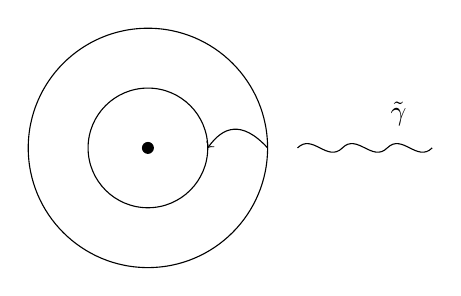
\begin{tikzpicture}[scale=0.95]
\fill (0,0) circle (0.08);
\draw (0,0) circle (0.8);
\draw (0,0) circle (1.6);
\draw[->] (1.6,0) .. controls (1.25,0.38) and (1.0,0.28) .. (0.8,0);
\draw (2.0,0) .. controls (2.2,0.2) and (2.4,-0.2) .. (2.6,0)
            .. controls (2.8,0.2) and (3.0,-0.2) .. (3.2,0)
            .. controls (3.4,0.2) and (3.6,-0.2) .. (3.8,0);
\node at (3.35,0.45) {$\tilde\gamma$};
\end{tikzpicture}

\caption{Radiative drop to a lower orbit. The board shows only emitted radiation; the photino label in the redraw is supplied from the transcript, not from a legible board inscription.}
\end{figure}

The point is not just that one exotic transition becomes allowed. The point is that the mechanism can happen again and again. Valence structure would collapse inward. What would accumulate near the nucleus would be something more like a Bose condensation of selectrons than an ordinary atom with well-separated shells. Whatever such a world would be, it would not support familiar chemistry.

The lecture is very direct about the conclusion. We do not live in an exactly supersymmetric world. One possible answer to the question ``why not?'' is simply that if supersymmetry were exact, we would not be here to ask. That is not a complete dynamical explanation, but it is a physically serious observation.

\section{Summary}

The lecture reaches supersymmetry by a sequence of concrete sign arguments. First, a \(2\pi\) rotation is topologically nontrivial, though \(4\pi\) is trivial. Second, a spin state may therefore return under \(2\pi\) only up to a sign, and for fermions that sign is negative. Third, exchange symmetry makes fermionic two-particle states anti-symmetric. Fourth, that anti-symmetry implies that a closed fermion loop contributes with an extra minus sign.

Once that much is in place, the supersymmetric idea is almost forced on us. If bosonic and fermionic corrections come with opposite signs, then matched boson-fermion partner pairs can cancel dangerous contributions to the vacuum energy and to boson self-energies. Exact matching is false in nature, so any realistic supersymmetry must be broken. But if it is broken too badly, it ceases to protect the Higgs sector. And if it were unbroken, ordinary chemistry would disappear. That is the balance the lecture leaves us with: supersymmetry is motivated precisely because exact supersymmetry is impossible for a world like ours.